\documentclass[11pt]{article}
\usepackage{geometry}                % See geometry.pdf to learn the layout options. There are lots.
\geometry{letterpaper}                   % ... or a4paper or a5paper or ... 
%\geometry{landscape}                % Activate for for rotated page geometry
%\usepackage[parfill]{parskip}    % Activate to begin paragraphs with an empty line rather than an indent
\usepackage{graphicx}
\usepackage{amssymb}
\usepackage{amsmath}
\usepackage{epstopdf}
\usepackage{hyperref}
\DeclareGraphicsRule{.tif}{png}{.png}{`convert #1 `dirname #1`/`basename #1 .tif`.png}


\graphicspath{
{/Users/Andy/Cruises_Research/Analysis/Andy_Pickering/eq14_patch_gamma/figures/}
{/Users/Andy/Cruises_Research/Analysis/Andy_Pickering/eq14_patch_gamma/figures/chi_eps_profiles_diffNprof_profavgs/zsm10m_fmax7Hz_respcorr0_fc_99hz_gamma20_nfft_128_screen_chi_1/}
{/Users/Andy/Cruises_Research/Analysis/Andy_Pickering/eq14_patch_gamma/figures/boot_eps_profiles_multprof/}
}

\title{Summary of $\chi$pod / Chameleon EQ14 Analysis}
\author{Andy Pickering}
%\date{}                                           % Activate to display a given date or no date



\begin{document}
\maketitle

\tableofcontents
\newpage



%~~~~~~~~~~~~~~~~~~~~~~~~~~~~~~~~~~~~~~~~~~~~~~~~~~~~~~~~~
\section{Overview}
%~~~~~~~~~~~~~~~~~~~~~~~~~~~~~~~~~~~~~~~~~~~~~~~~~~~~~~~~~


\begin{itemize}

\item This document is an attempt to provide an overview/summary of what i've found in my $\chi$pod analysis so far. 

\item The motivation/goal for all this work is to show if /how well the CTD-$\chi$pod method works for estimating $\chi$,$\epsilon$, $K_T$, etc from fast temperature (thermistor) profiles. The idea is to deploy $\chi$pods on regular CTD casts on WOCE/CLIVAR cruises etc. to making mixing measurements.

\item Before dealing with all the issues with the CTD deployments (depth loops, entrained water, rosette-induced turbulence etc.), I wanted to verify that the method itself worked w/out these complications. 

\item The Chameleon microstructure profiler has both thermistor and shear probes, so this seemed like an ideal way to test the method. I would apply the $\chi$pod method to the chameleon thermistor data only ($\chi_{\chi},\epsilon_{\chi}$), and compare to the `true' results computed using the shear probes ($\chi$,$\epsilon$).

\end{itemize}







\clearpage
%~~~~~~~~~~~~~~~~~~~~~~~~~~~~~~~~~~~~~~~~~~~~~~~~~~~~~~~~~
\section{Data and Processing}
%~~~~~~~~~~~~~~~~~~~~~~~~~~~~~~~~~~~~~~~~~~~~~~~~~~~~~~~~~


\begin{itemize}

\item Data are from Chameleon profiles near the equator during the `EQ14' experiment. On my laptop, they are located in the folder: \newline 
\verb+/Cham_Eq14_Compare/Data/chameleon/processed/+

\item Sally shared w/ me Chameleon data that she and Jim processed. I ended up re-processing it using a smaller fmax (7Hz) because it looked like the thermistor spectra rolled off much lower than the normally-assumed 32Hz. These data are located at: \newline
\verb+/Cham_Eq14_Compare/Data/chameleon/processed_AP_7hz/+

\item  The $\chi$pod method is applied to Chameleon profiles (thermistor only, not shear probe) from EQ14 in \verb+ComputeChi_Chameleon_Eq14.m+

\item The noise floor of Chamleon $\epsilon$ was determined to be $log_{10}[\epsilon]=-8.5$. Values below this threshold were discarded. $\chi$pod values below this threshold were also discarded, in order to make a valid comparison. An upper limit of $log_{10}[\epsilon]=-5$ (determined by Jim?) was also applied.

\item Data including surface convection was identified and excluded in the analysis. The mixed layer depth was identified (\verb+Identify_mixedlayer_eq14.m+) using a criteria of $\sigma -\simga_{surface}=0.04$. This depth is shown in figures \ref{chi_overview} and \ref{eps_overview}.

\item \verb+Make_Overview_Plots.m+ Makes the figures in this document.

\end{itemize}









\clearpage
%~~~~~~~~~~~~~~~~~~~~~~~~~~~~~~~~~~~~~~~~~~~~~~~~~~~~~~~~~
\section{Results}
%~~~~~~~~~~~~~~~~~~~~~~~~~~~~~~~~~~~~~~~~~~~~~~~~~~~~~~~~~


%~~~~~~~~~~~~~~~~~~
\subsection{Overview}
%~~~~~~~~~~~~~~~~~~



\begin{itemize}

\item Both $\chi_{\chi}$ and $\epsilon_{\chi}$ appear to capture the depth and time structure of $\chi$ and $\epsilon$ well (Figures \ref{chi_overview},\ref{eps_overview}).


\end{itemize}



% misc_Appr14.m
\begin{figure}[htbp]
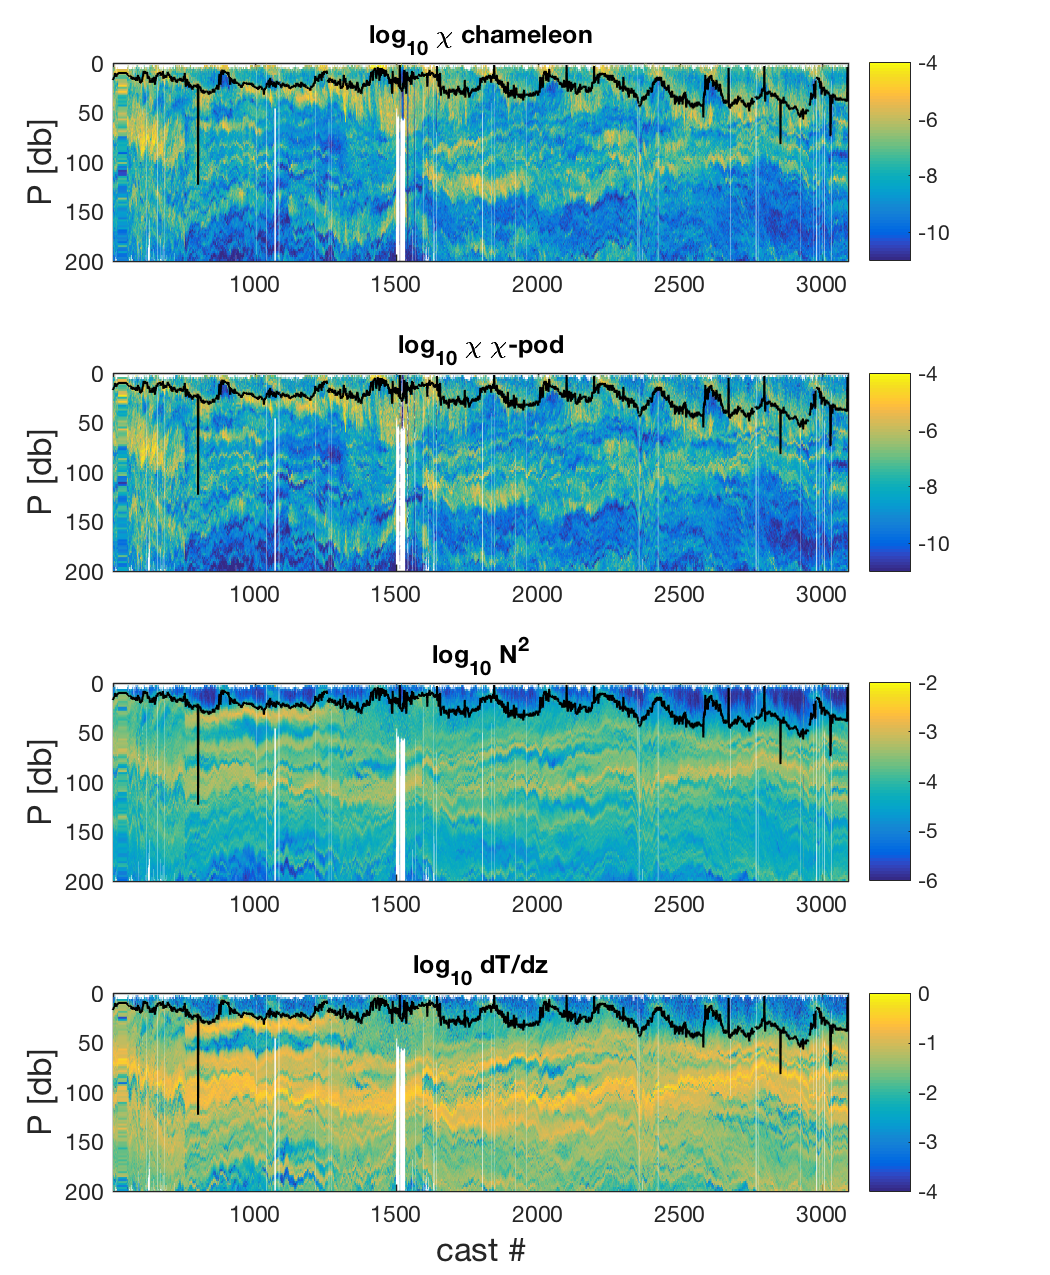
\includegraphics[scale=0.8]{eq14_Pcolor_BothChi_N2_Tz_screen_chi_1_zsm1m_fmax7Hz_respcorr0_fc_99hz_gamma20.png}
\caption{Comparison of $\chi$ from chameleon method and chi-pod method, for EQ14 chameleon profiles. Each profile was averaged in 2m bins.  Black line shows shows convective regions excluded in further analysis.}
\label{chi_overview}
\end{figure}

\begin{figure}[htbp]
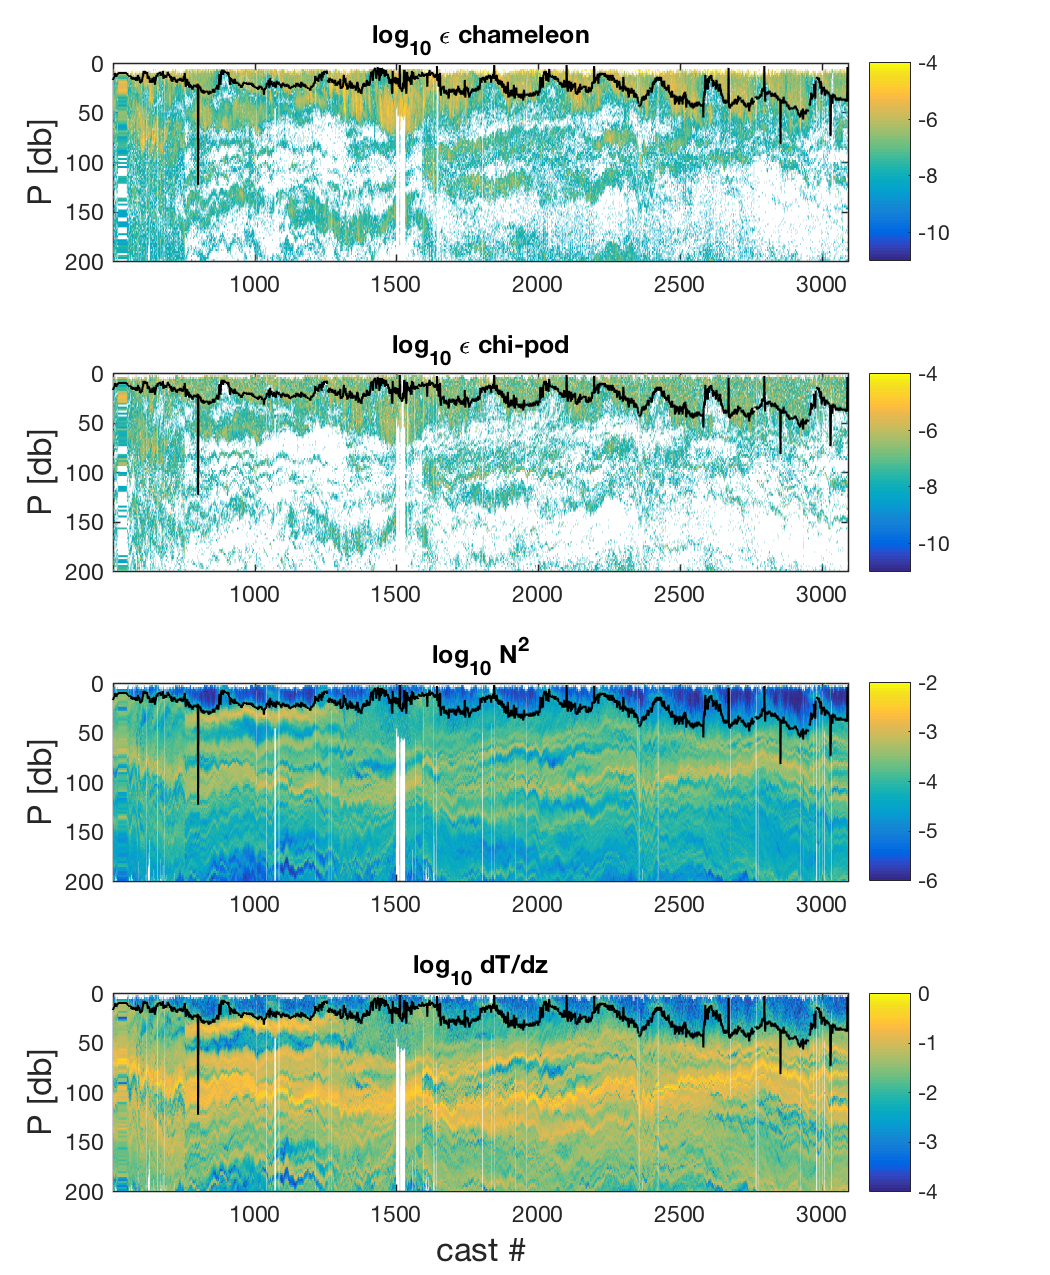
\includegraphics[scale=0.8]{eq14_Pcolor_BothEps_N2_Tz_screen_chi_1_zsm1m_fmax7Hz_respcorr0_fc_99hz_gamma20.png}
\caption{Comparison of $\epsilon$ from chameleon method and chi-pod method, for EQ14 chameleon profiles. Each profile was averaged in 2m bins.  Values of $\epsilon_{\chi}$ and $\epsilon$ below chameleon noise floor ($log_{10}[\epsilon]=-8.5$) have been nan'd out. Black line shows shows convective regions excluded in further analysis.}
\label{eps_overview}
\end{figure}




\clearpage
%~~~~~~~~~~~~~~~~~~~~~~~~~~~~~~~~~~~~~~~~
\subsection{Comparing individual estimates of $\epsilon$}
%~~~~~~~~~~~~~~~~~~~~~~~~~~~~~~~~~~~~~~~~

\begin{itemize}

\item Both $\chi_{\chi}$ and $\epsilon_{\chi}$ are biased low (Figures \ref{2DchamVschi},\ref{histchamVschi}); the $\epsilon_{\chi}$ bias is larger (more negative).

\item The bias in $\chi$ is relatively constant with depth; the bias in $\epsilon$ is more negative at shallower depths (Figure \ref{chamVschivsP}).

\end{itemize}


%  plot of $\chi$pod vs cham for chi and eps
\begin{figure}[htbp]
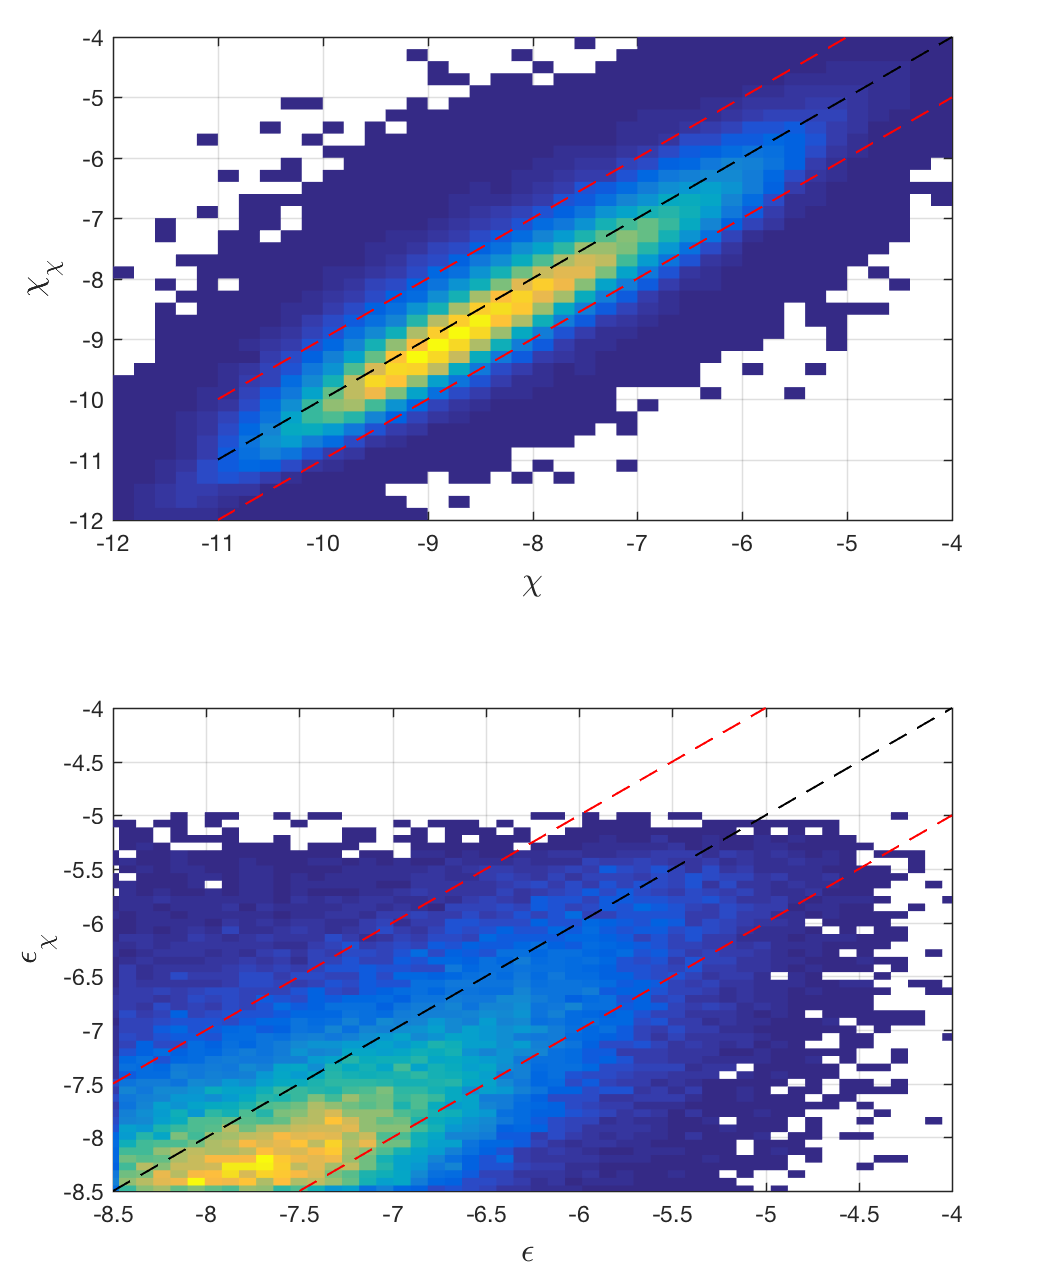
\includegraphics[scale=0.8]{eq14_chamVschipod_screen_chi_1_zsm1m_fmax7Hz_respcorr0_fc_99hz_gamma20.png}
\caption{Comparison of $\chi$ (top) and $\epsilon$ (lower) from chameleon method and chi-pod method, for EQ14 chameleon profiles. Each profile was averaged in 2m bins.  Values of $\epsion$ below chameleon noise floor ($log_{10}[\epsilon]=-8.5$) have been nan'd out. Black line is 1:1, red lines are $+/-$ order of magnitude. }
\label{2DchamVschi}
\end{figure}


%  plot of $\chi$pod vs cham for chi and eps
\begin{figure}[htbp]
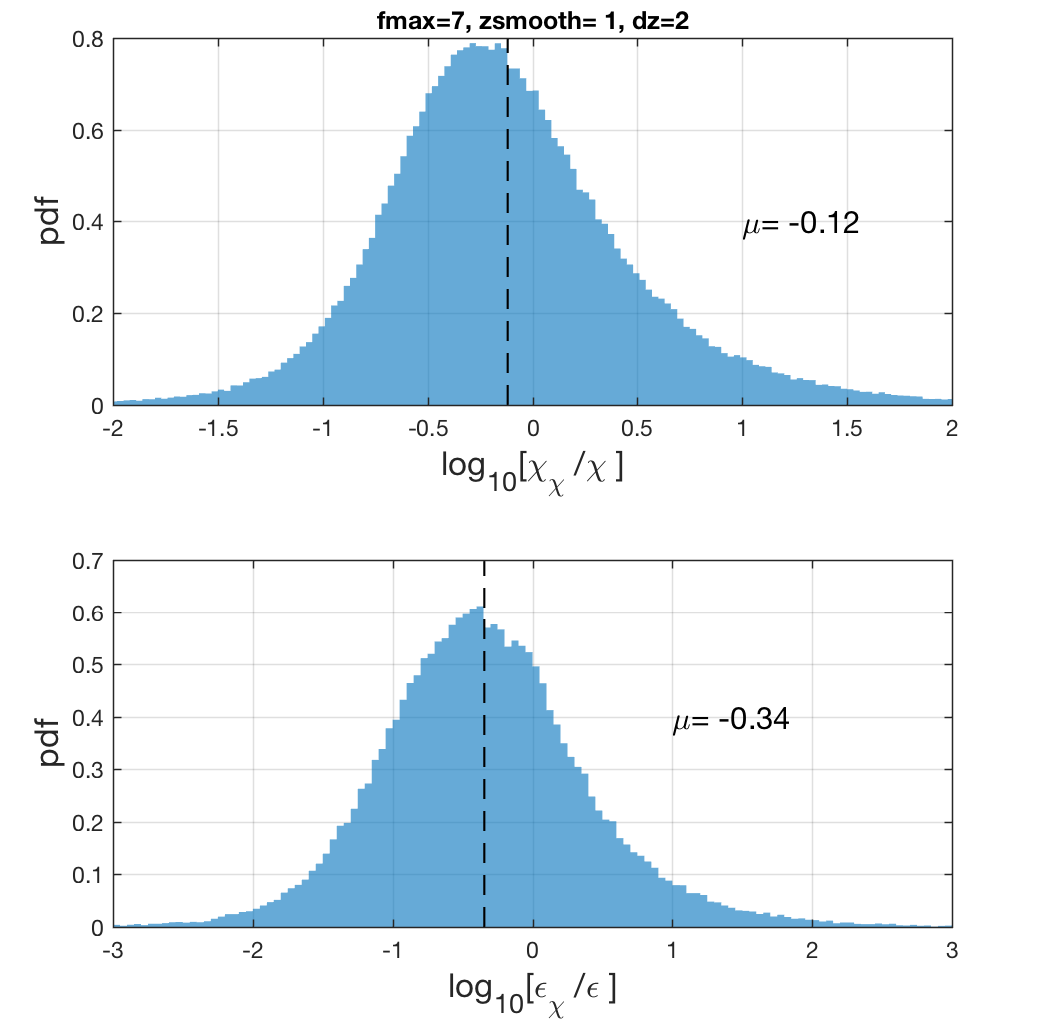
\includegraphics[scale=0.8]{eq14_2mbinned_eps_ratios_screen_chi_1_screenml_1_zsm1m_fmax7Hz_respcorr0_fc_99hz_gamma20.png}
\caption{Histograms of the ratios of $\chi_{\epsilon}/\chi$ (top) and $\epsilon_{\chi}/\epsilon$ (lower) .}
\label{histchamVschi}
\end{figure}



\begin{figure}[htbp]
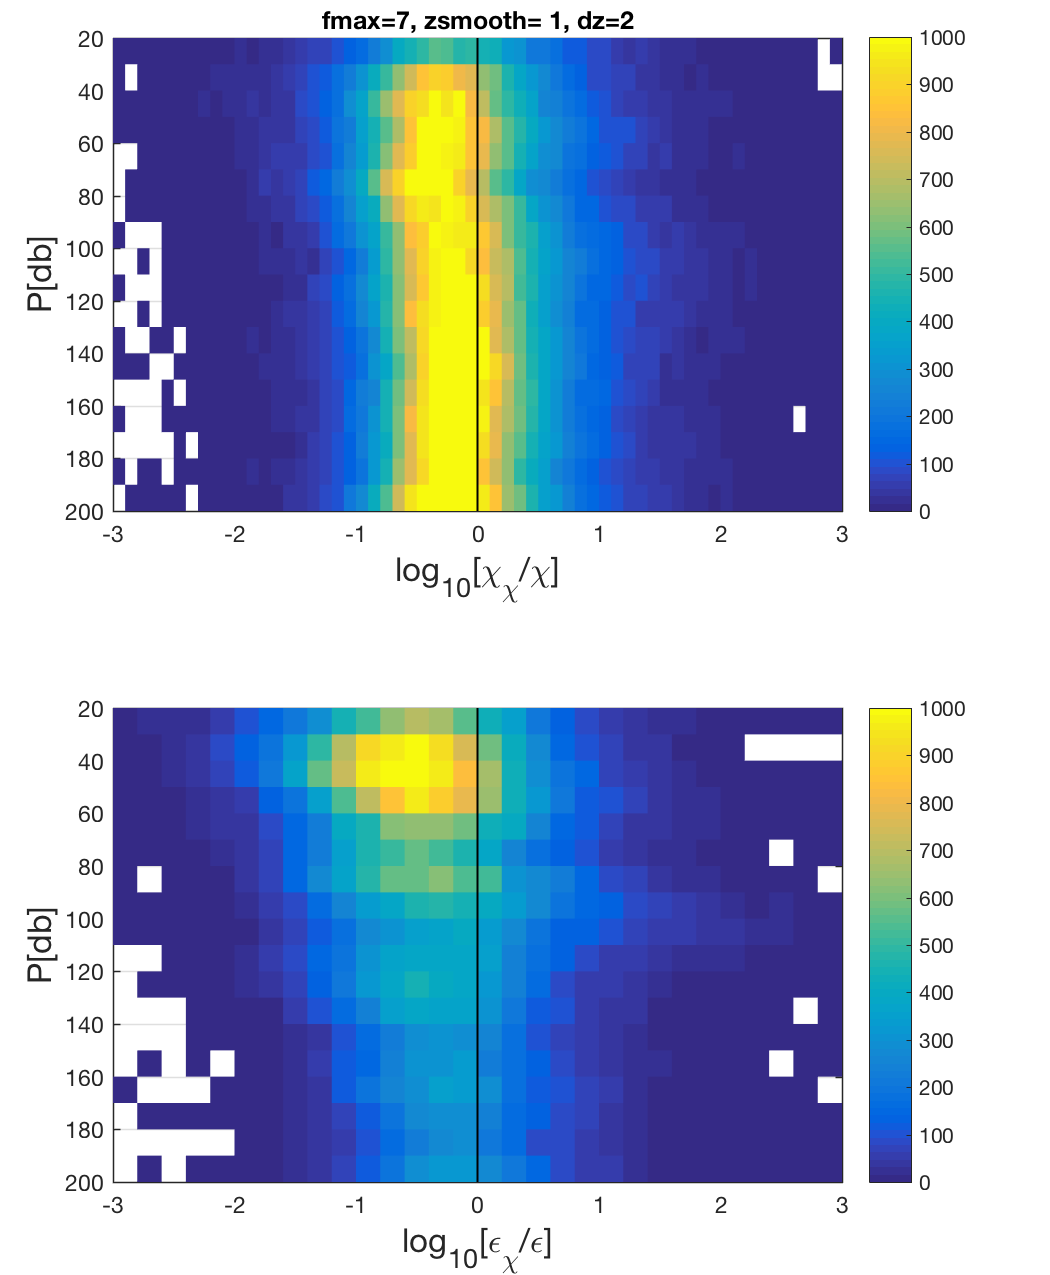
\includegraphics[scale=0.8]{eq14_chi_eps_Vs_P_2Dhist_screen_chi_1_zsm1m_fmax7Hz_respcorr0_fc_99hz_gamma20.png}
\caption{ 2D histograms of ratios $\chi_{\chi}$ and $\epsilon_{\chi}$ ratios vs depth.}
\label{chamVschivsP}
\end{figure}





\clearpage
%~~~~~~~~~~~~~~~~~~~~~~~~~~~~~~~~~~~~~~~~
\subsection{Normalized eps vs chi plots}
%~~~~~~~~~~~~~~~~~~~~~~~~~~~~~~~~~~~~~~~~

Assuming that
\begin{equation}
\gamma=\frac{N^2 \chi}{2\epsilon<T_z>^2}
\end{equation}
, plotting [$\chi/t_{z}^{2}$] vs [$\epsilon/N\^2$] should follow a straight line with slope equal to $2\gamma$. Chameleon data from EQ14 tend to fall near $\gamma=0.05$ (Figure \ref{chiepsnorm}).


\begin{figure}[htbp]
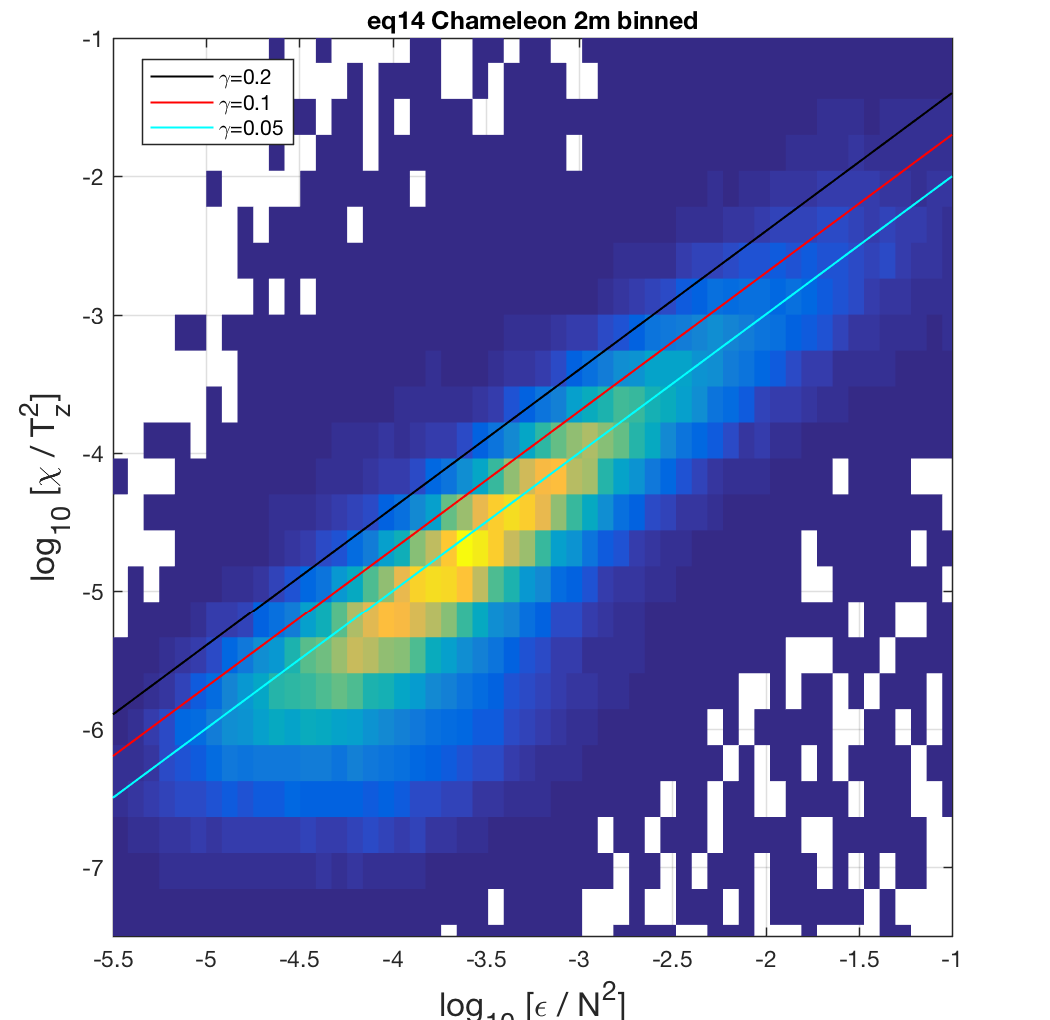
\includegraphics[scale=0.8]{eq14_2mbinned_eps_vs_chi_normalized_zsm1m_fmax7Hz_respcorr0_fc_99hz_gamma20.png}
\caption{EQ14: 2m binned  chameleon $\epsilon/N\^2$ vs $\chi/t_{z}^{2}$. Lines show different values of $\gamma$. Values of $\epsilon$ below noise floor ($log_{10}\epsilon<-8.5$) are discarded also.}
\label{chiepsnorm}
\end{figure}






\clearpage
%~~~~~~~~~~~~~~~~~~~~~~~~~~~~~~~~~~~~~~~~
\subsection{Averaging multiple profiles of $\epsilon$}
%~~~~~~~~~~~~~~~~~~~~~~~~~~~~~~~~~~~~~~~~


\begin{itemize}

\item Averaging over multiple profiles reduces the bias in both $\chi$ and $\epsilon$ (Figures \ref{2Dhistdiffprof},\ref{histdiffprof}).

\item Averaging 10 profiles together seems to give the smallest bias.

\end{itemize}


Figure \ref{prof_avg_ex} shows one example. 


\begin{figure}[htbp]
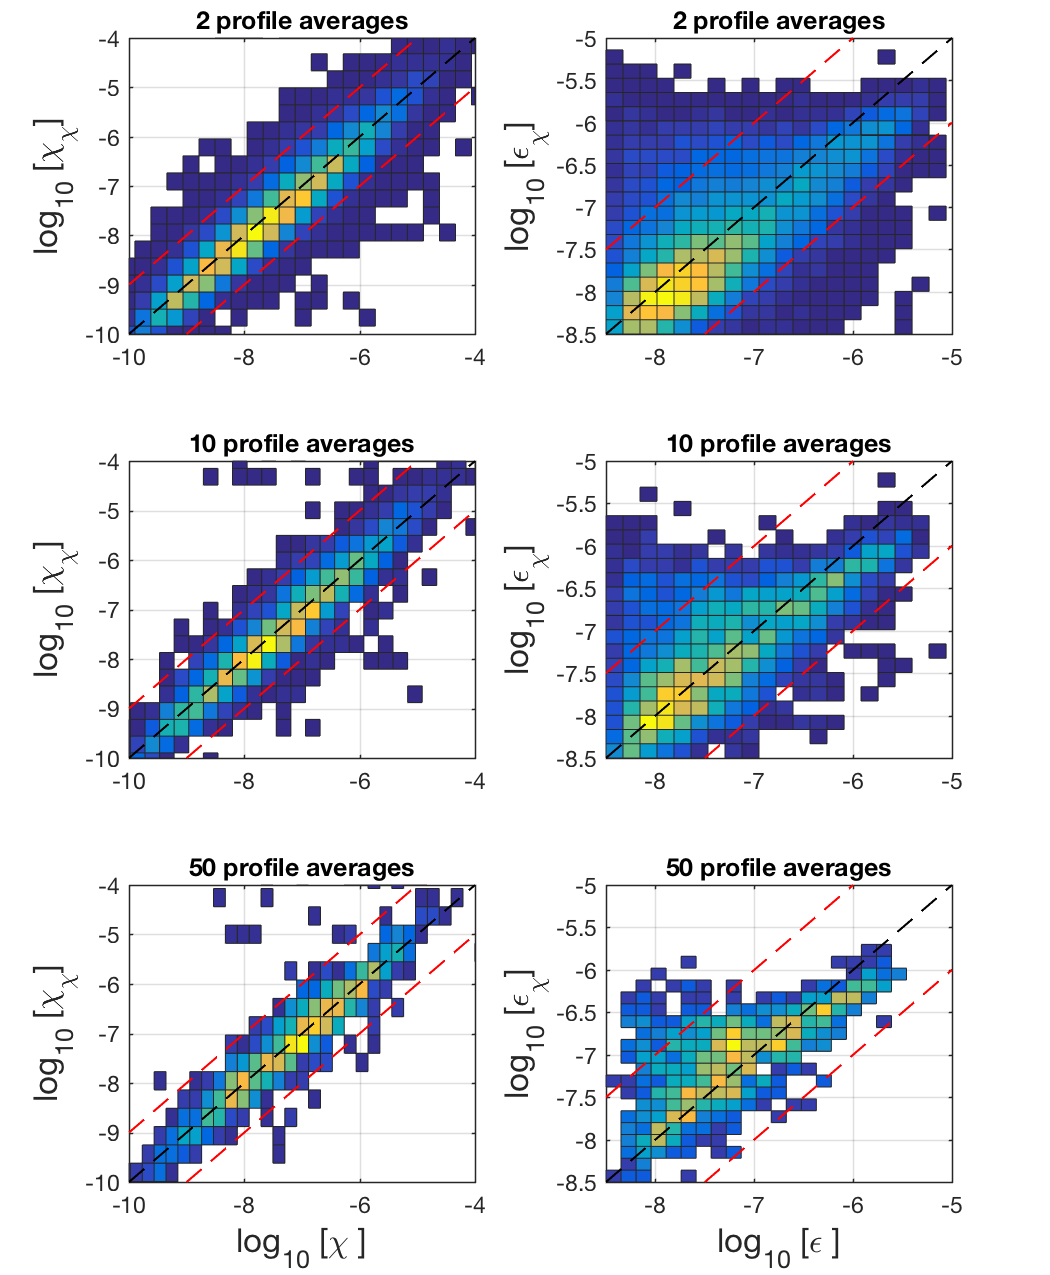
\includegraphics[scale=0.8]{eq14_chiVscham_chiANDeps_diff_prof_avg_screen_chi_1_zsm1m_fmax7Hz_respcorr0_fc_99hz_gamma20.png}
\caption{2D Histograms of $\chi_{chi}$ vs $\chi$ (left) and $\epsilon_{\chi}$ vs $\epsilon$ (right) for different numbers of profiles averaged. }
\label{2Dhistdiffprof}
\end{figure}


\begin{figure}[htbp]
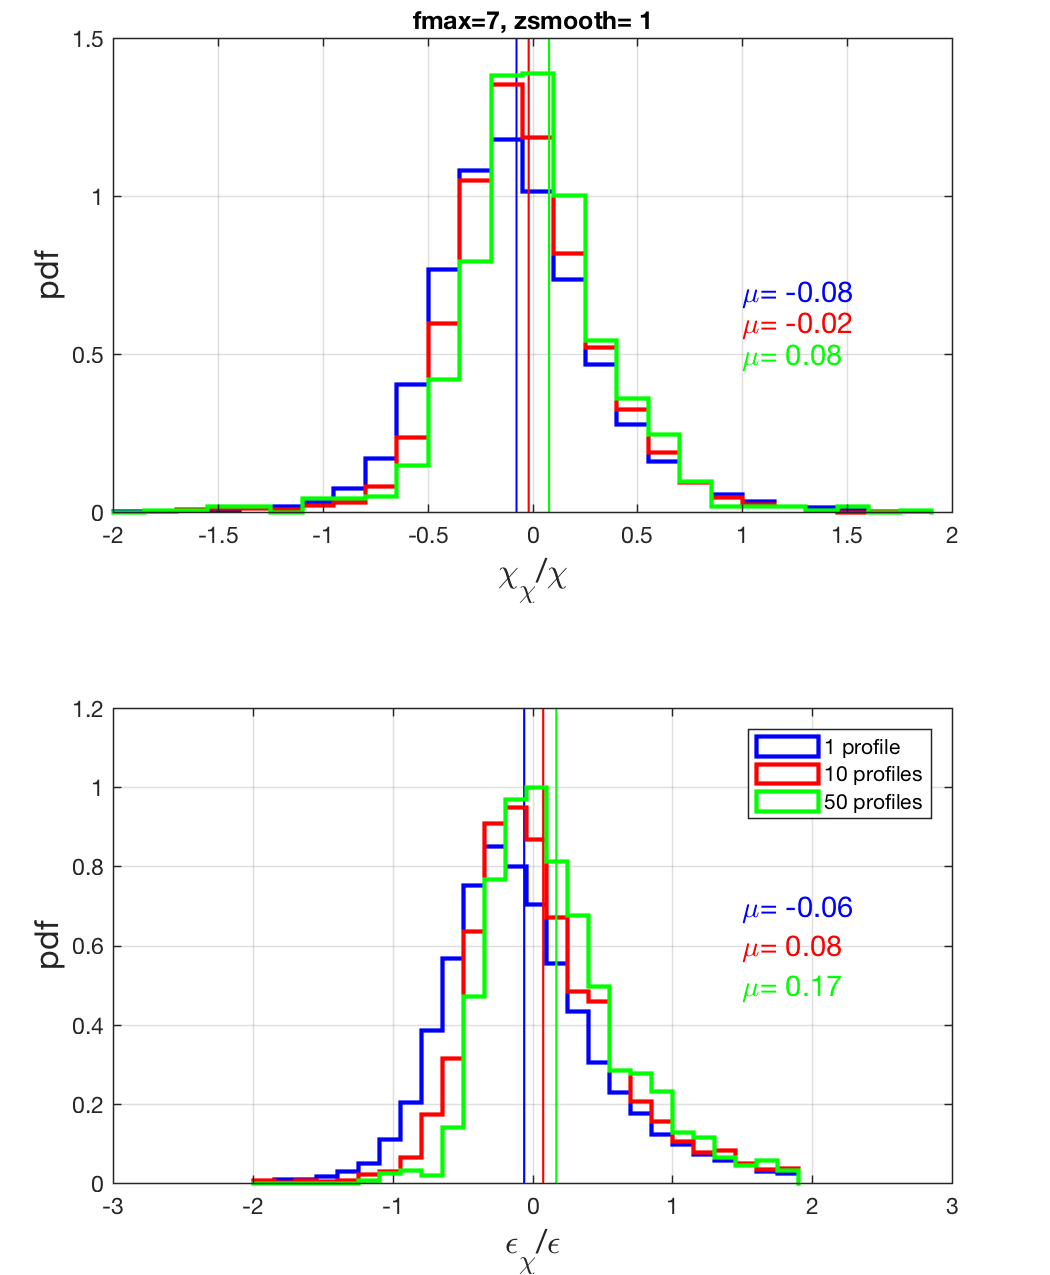
\includegraphics[scale=0.8]{eq14_eps_ratio_hist_diff_prof_avg_zsm1m_fmax7Hz_respcorr0_fc_99hz_gamma20.png}
\caption{(log10) Ratio of $\epsilon_{\chi}/\epsilon$ for different numbers of profiles averaged. Consecutive chunks of N profiles were averaged, and then (normalized) histogram of the ratios was plotted. Vertical lines and numbers to right are mean of $log_{10}[\epsilon_{\chi}/\epsilon]$ for each distribution. }
\label{histdiffprof}
\end{figure}


\begin{figure}[htbp]
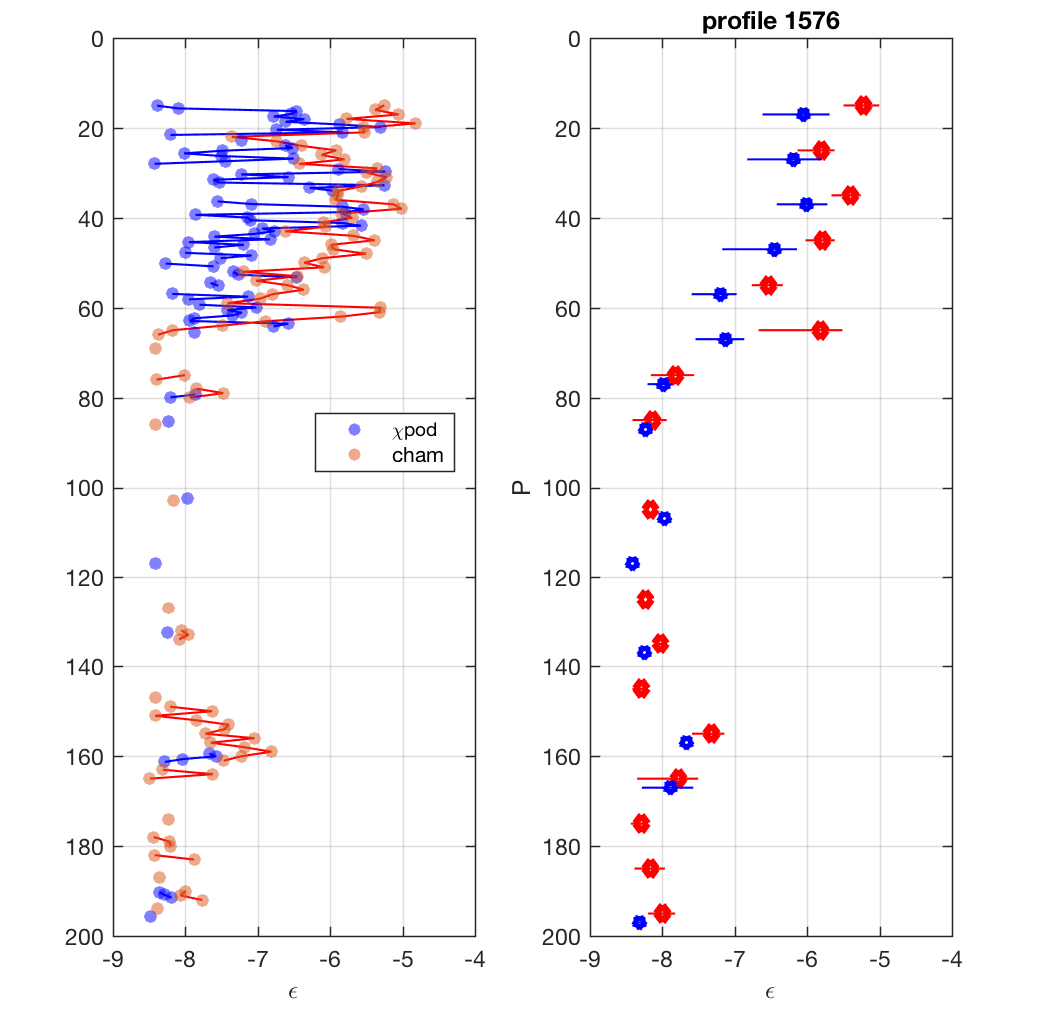
\includegraphics[scale=0.8]{eps_boot_prof_cnum_1576.png}
\caption{Example of averaging multiple profiles together. Left panels show a single profile from chamleeon and chi-pod method. Right panel shows bootstrap average of 5 profiles, averaged in 10m depth bins, with 95\% confidence intervals. Data in mixed layer and shallower than 20m have been excluded.}
\label{prof_avg_ex}
\end{figure}




\clearpage
%~~~~~~~~~~~~~~~~~~~~~~~~~~~~~~~~~~~~~~~~
\subsection{Averaging over different-sized depth bins}
%~~~~~~~~~~~~~~~~~~~~~~~~~~~~~~~~~~~~~~~~


\begin{itemize}

\item Averaging over large depth bins reduces the bias in both $\chi$ and $\epsilon$ (Figures \ref{2Dhistdiffdz},\ref{histdiffdz}).

\end{itemize}


\begin{figure}[htbp]
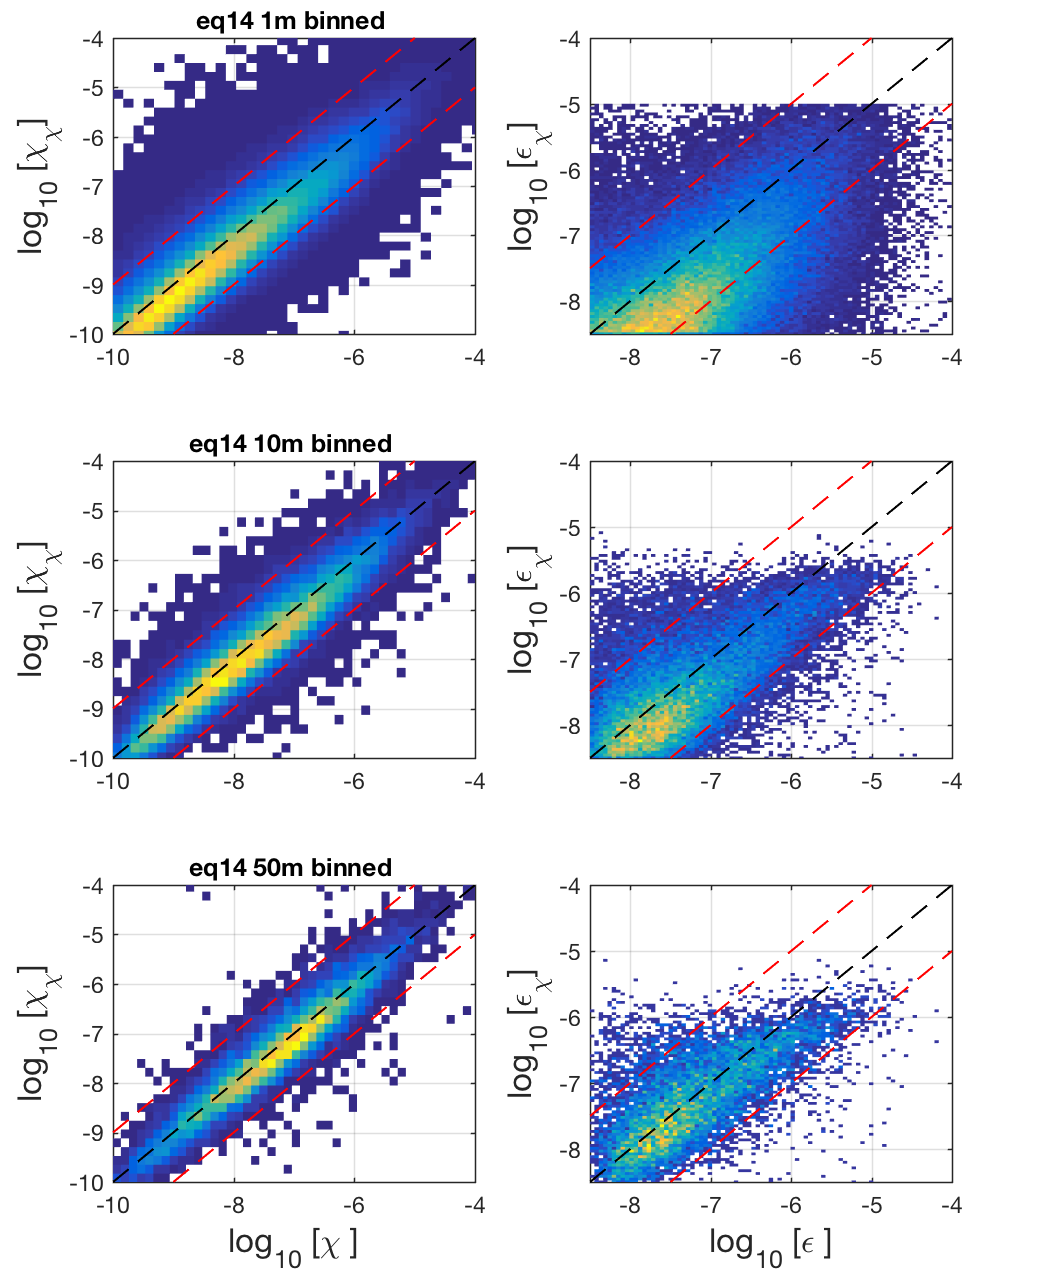
\includegraphics[scale=0.8]{eq14_chiVscham_chiANDeps_diff_dz_screen_chi_1_zsm1m_fmax7Hz_respcorr0_fc_99hz_gamma20.png}
\caption{2D Histograms of $\chi_{chi}$ vs $\chi$ (left) and $\epsilon_{\chi}$ vs $\epsilon$ (right) averaged over different size depth bins}
\label{2Dhistdiffdz}
\end{figure}



\begin{figure}[htbp]
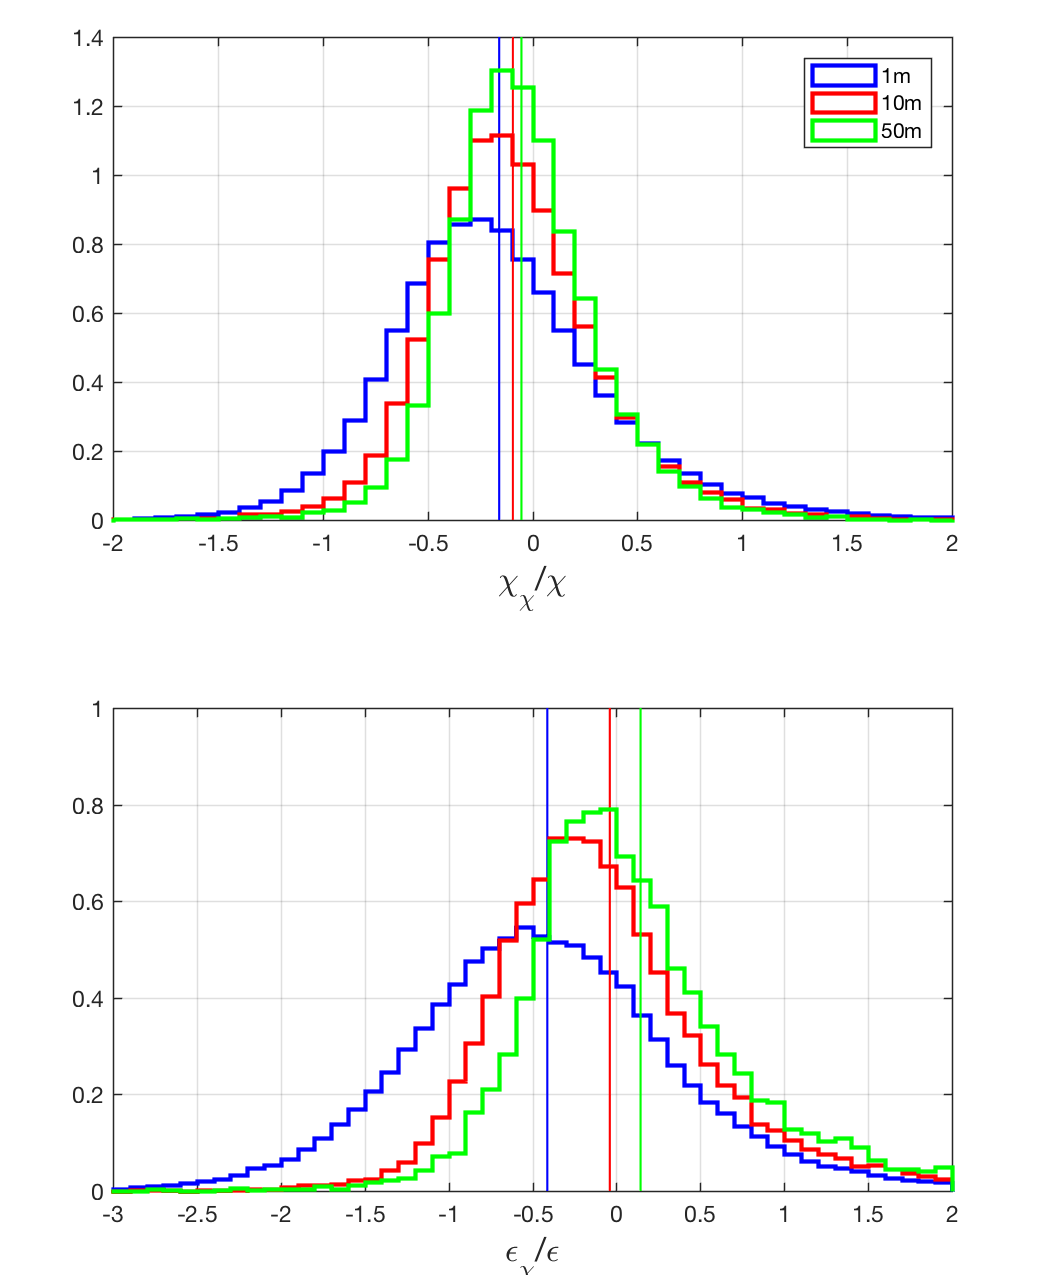
\includegraphics[scale=0.8]{eq14_chiVscham_hist_diff_dz_screen_chi_1_zsm1m_fmax7Hz_respcorr0_fc_99hz_gamma20.png}
\caption{Histogram of log10 of ratio $\epsilon_{\chi}/\epsilon$ for different amounts of vertical averaging. Vertical lines are mean of $log_{10}[\epsilon_{\chi}/\epsilon]$ for each distribution.}
\label{histdiffdz}
\end{figure}









\clearpage
%~~~~~~~~~~~~~~~~~~~~~~~~~~~~~~~~~~~~~~~~
\subsection{$\gamma$ computed from averaged quantities}
%~~~~~~~~~~~~~~~~~~~~~~~~~~~~~~~~~~~~~~~~

If we compute gamma from time-averaged $N^2,T_z,\chi,\epsilon$ do we get $\gamma=0.2$ (or a different gamma)? Estimates from the averaged data are larger (Figure \ref{gambox_eq14}) but still slightly less than 0.2 .

\begin{figure}[htbp]
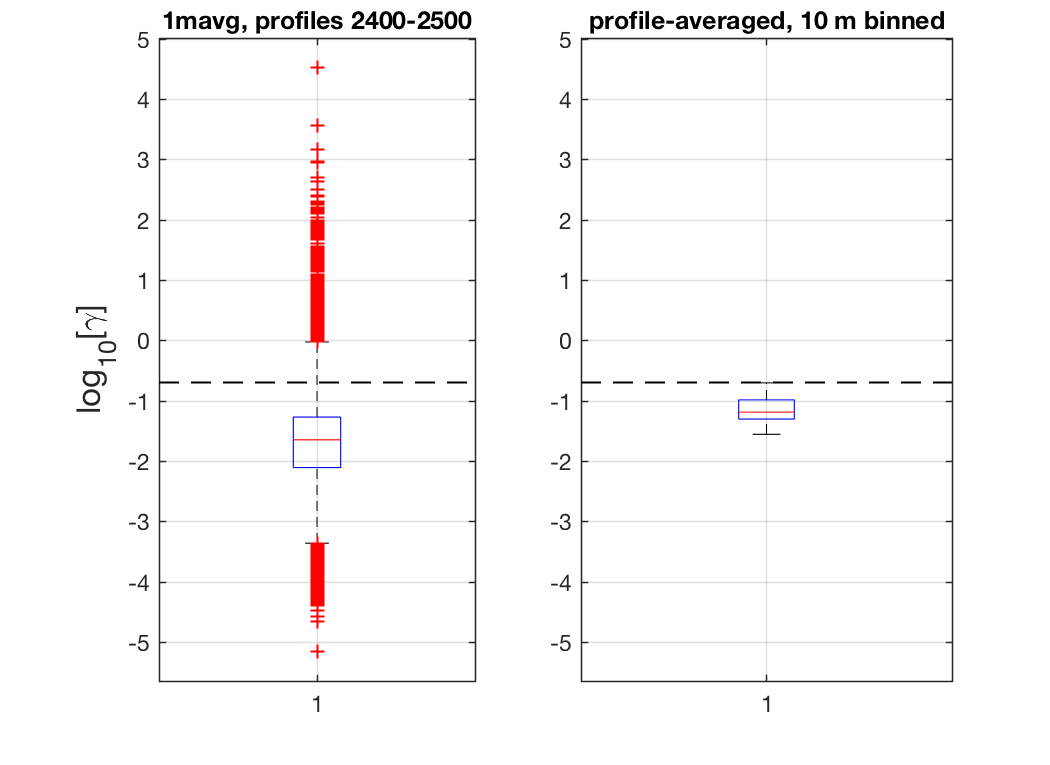
\includegraphics[scale=0.8]{eq14_gamma_point_avg_box_10mbinned.png}
\caption{Boxplots of $log_{10}[\gamma]$ for a set of profiles from EQ14. Left is for all 1m avg data. Right is for data from all profiles averaged in 10m bins. Horizontal dashed line indicates $\gamma=0.2$.}
\label{gambox_eq14}
\end{figure}








%~~~~~~~~~~~~~~~~~~~~~~~~~~~~~~~~~~~~~~~~~~~~~~~~~~~~~~~~~
\end{document}  
%~~~~~~~~~~~~~~~~~~~~~~~~~~~~~~~~~~~~~~~~~~~~~~~~~~~~~~~~~
%~~~~~~~~~~~~~~~~~~~~~~~~~~~~~~~~~~~~~~~~~~~~~~~~~~~~~~~~~
%~~~~~~~~~~~~~~~~~~~~~~~~~~~~~~~~~~~~~~~~~~~~~~~~~~~~~~~~~


